%=========================================================================
% (c) 2011, 2012 Josef Lusticky

\section{Network and timestamps}\label{sec:ntp-network}
The network specification of NTP defines
the protocol to use the User Datagram Protocol (UDP) on port number 123~\cite{ianna-ports,rfc5905}.
Reliable message delivery such as TCP can actually make the delivery of
NTP packet less reliable since retries
would increase the delay value and other errors~\cite{rfc5905}.
This is mostly due to overhead of communication with TCP on the transport layer.

NTP handles the time through timestamps - a record of time.
An NTP timestamp has two fields: the seconds field expressing the number of seconds
and the fraction field expressing fraction of a second~\cite{rfc5905}.
All NTP timestamps are represented in 2-complement format, with
bits numbered in big-endian fashion from zero starting at the left, or high-order position~\cite{rfc5905}.
There are two timestamp formats in the NTP packet structure:
long 64-bit and short 32-bit as shown in figure~\ref{fig:ntp-timestamps}.
The 64-bit long timestamp used by NTP consists of a 32-bit unsigned seconds
field spanning $2^{32}$ seconds (approx. 136 years from 1900 to 2036) and a 32-bit fraction field resolving
$2^{-32}$ seconds (approx. 232 picoseconds)~\cite{rfc5905}.
The short 32-bit timestamp includes a 16-bit unsigned seconds field
and a 16-bit fraction field.

\begin{figure}
	\centering
	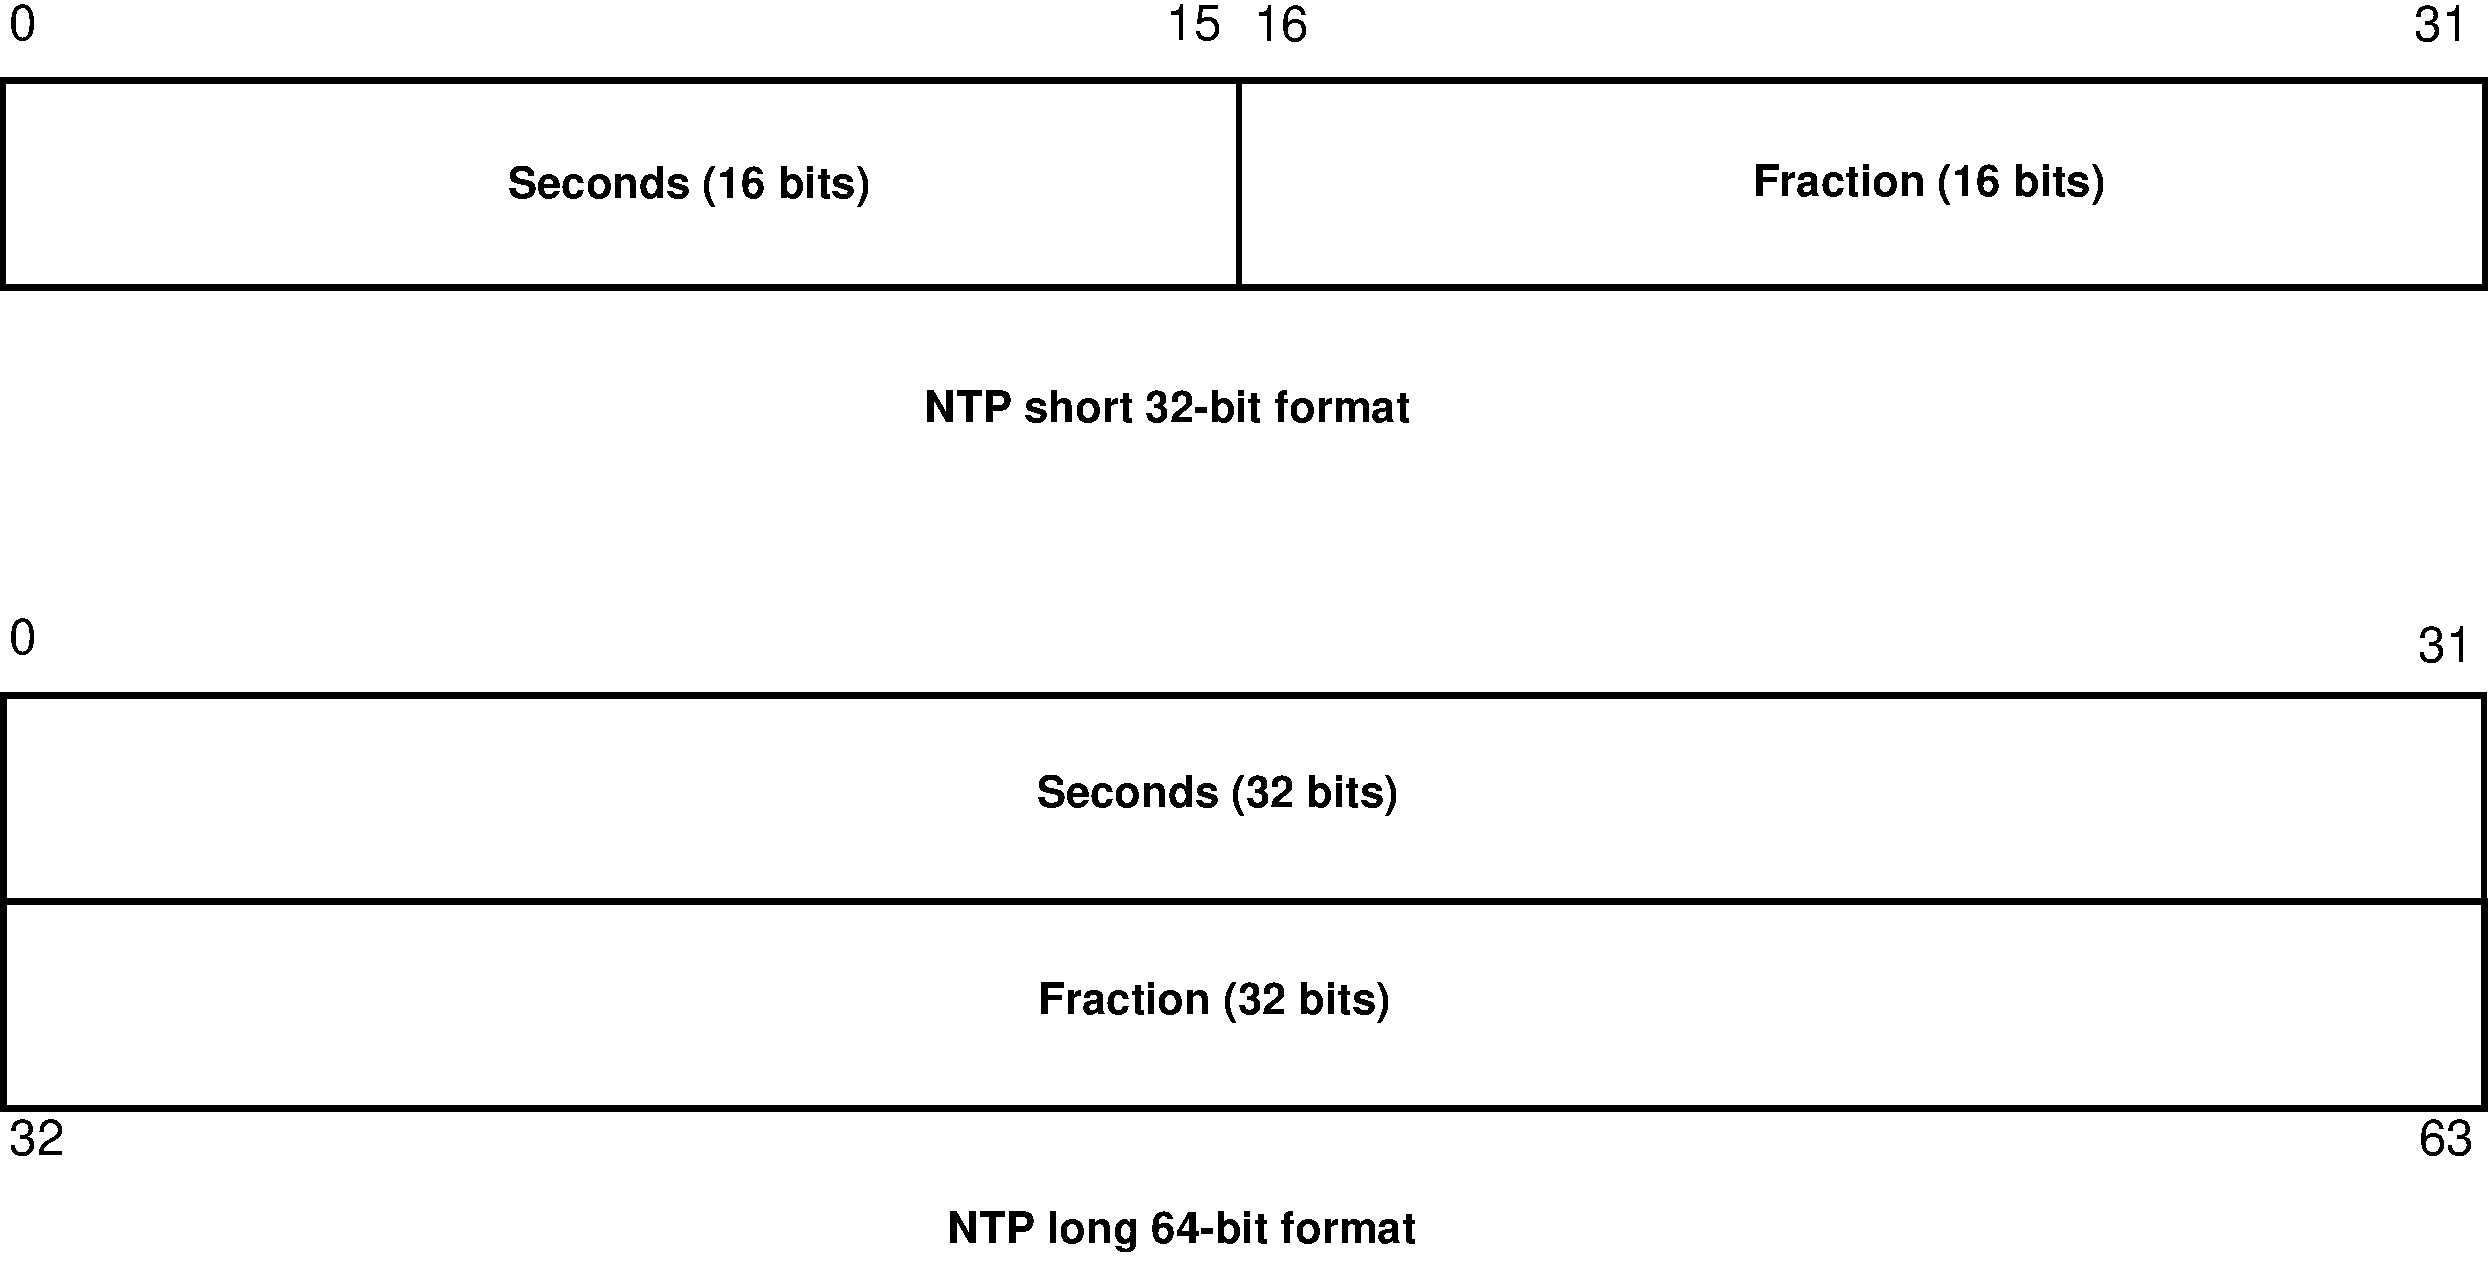
\includegraphics[width=13cm,keepaspectratio]{fig/ntp-timestamps.pdf}
	\caption{Time formats used in NTP packet}
	\label{fig:ntp-timestamps}
	\bigskip
\end{figure}

Besides these two, there is one more NTP timestamp format - the 128-bit NTP Date format.
It includes a 64-bit signed seconds field and 64-bit fraction field.
For convenience in mapping between formats,
the seconds field is divided into 32-bit Era Number field
and 32-bit Era Offset field.
This 128-bit NTP Date format is however not transmitted over the network
and is only used where sufficient storage and word size is available~\cite{rfc5905}.
There is practically no need of knowing about this format for embedded systems
at least until year 2036, when 64-bit long timestamp wraps around and
the Era Number will be incremented from zero to one.
But strictly speaking, the NTP timestamp is the truncated NTP Date format~\cite{rfc5905}.

\begin{figure}
	\centering
	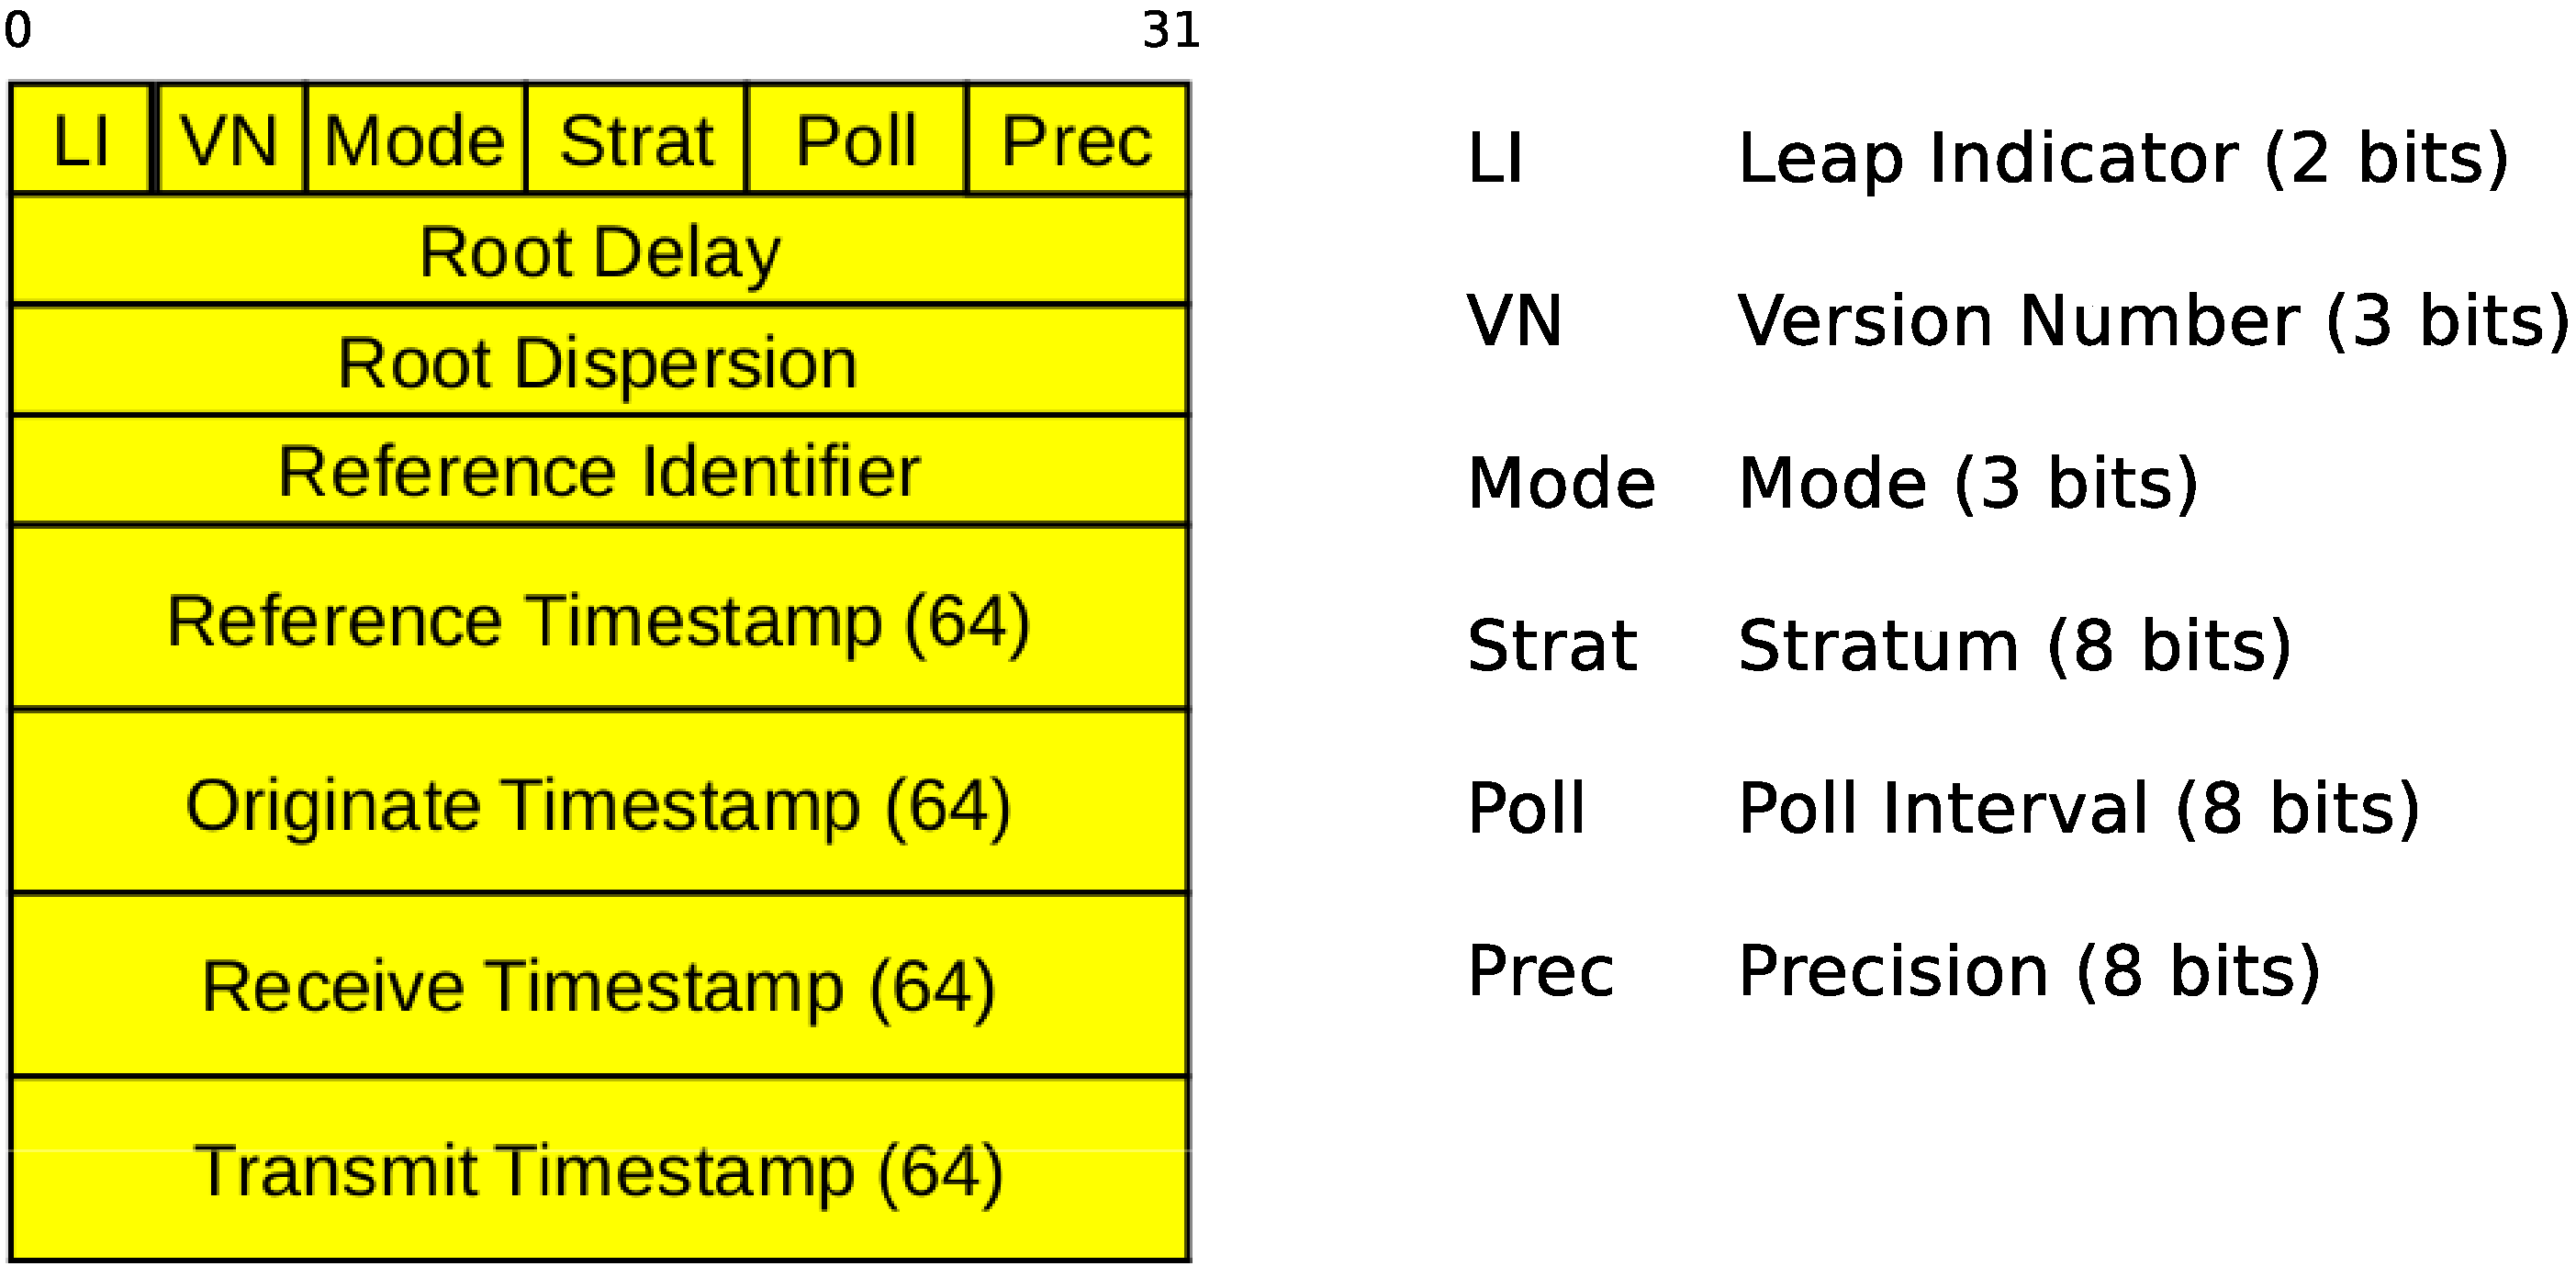
\includegraphics[width=9cm,keepaspectratio]{fig/ntp-packet.pdf}
	\caption{Basic NTP packet structure (source:~\cite{ntp-arch})}
	\label{fig:ntp-packet}
	\bigskip
\end{figure}

Standard NTP packet structure without extension fields and
Autokey security protocol is shown in figure~\ref{fig:ntp-packet}.
This structure is 48 bytes long and contains the following thirteen fields:
\begin{itemize}
\item
Leap Indicator is a 2-bit integer warning of an impending leap
second to be inserted or deleted in the last minute of the current month~\cite{rfc5905}.
\item
Version Number is a 3-bit integer representing the NTP
version number, currently~4.
\item
Mode is a 3-bit integer representing protocol mode.
This is the only field distinguishing between server and client in NTP.
In the client-server communication model, the client sets this field to value 3 (client) in the request,
and the server sets it to value 4 (server) in the response.
In broadcast communication model, the server sets this field to value 5 (broadcast).
Other modes are not used by SNTP servers and clients~\cite{rfc4330}.
\item
Stratum is an 8-bit integer representing the stratum as described in section~\ref{sec:ntp-topology}.
If the Stratum field is 0, which implies unspecified or invalid, the
Reference Identifier field can be used to convey messages useful for
status reporting and access control.
These are called Kiss-o'-Death (KoD)
packets and the ASCII messages they convey are called kiss codes~\cite{rfc5905}.
\item
Poll is an 8-bit signed integer representing the maximum interval between
successive messages, in log2 seconds.
Suggested default limits for minimum and maximum poll intervals are 6 and 10, respectively~\cite{rfc5905}.
\item
Precision is an 8-bit signed integer representing the precision of the
system clock, in log2 seconds.
For instance, a value of -20
corresponds to a precision of about one microsecond ($2^{-20}$~s)~\cite{rfc5905}.
\item
Root Delay is short 32-bit NTP timestamp expressing
total round-trip delay to the reference clock~\cite{rfc5905}.
\item
Root Dispersion is short 32-bit NTP timestamp expressing
total dispersion to the reference clock~\cite{rfc5905}.
\item
Reference Identifier is a 32-bit code identifying the particular server used for synchronisation
or reference clock.
For packet stratum 0, this is a four-character ASCII string called kiss code.
Kiss codes are particularly used by the server to tell the client to stop sending packets or
to increase its polling interval.
For stratum 1, this is a four-octet, left-justified, zero-padded ASCII
string assigned to the reference clock (e.g. "GPS" when synchronising against Global Position System clock).
Above stratum 1, this is the reference identifier of the server used for synchronisation
and can be used by the client together with stratum field to detect loops in the NTP hierarchy.
If communicating over IPv4, the identifier is IPv4 address.
If communicating over IPv6, it is the first four octets of the MD5 hash of the IPv6 address~\cite{rfc5905}.
\item
Reference Timestamp is long 64-bit NTP timestamp expressing the time
when the system clock was last synchronised against reference clock~\cite{rfc5905}.
\item
Originate Timestamp (or Origin Timestamp) is long 64-bit NTP timestamp expressing the time
at the client when the request departed for the server~\cite{rfc5905}.
Originate Timestamp field is copied
unchanged by the server from Transmit Timestamp field of the client's request.
It is important that the server copies this field intact,
as the NTP client uses it to check the server's response.
\item
Receive Timestamp is long 64-bit NTP timestamp expressing the time
at the server when the request arrived from the client~\cite{rfc5905}.
\item
Transmit Timestamp is long 64-bit NTP timestamp expressing the time
at the server when the response left for the client~\cite{rfc5905}.
\end{itemize}

The short 32-bit timestamp format is used for Root Dispersion and Root Delay fields,
because they do not need the scope and precision of the long 64-bit timestamp format.
The common unicast communication scenario is shown in figure~\ref{fig:ntp-client-server}
for better understanding of the NTP packet filling process and meaning of
Reference (ref), Originate (org), Receive (rec) and Transmit (xmt) timestamps.
Please note that this figure shows only communication mode and
timestamps used by NTP for local clock offset and round-trip delay calculation.
Algorithms used for such calculations are described in section~\ref{sec:ntp-algorithms}.

\begin{figure}
	\centering
	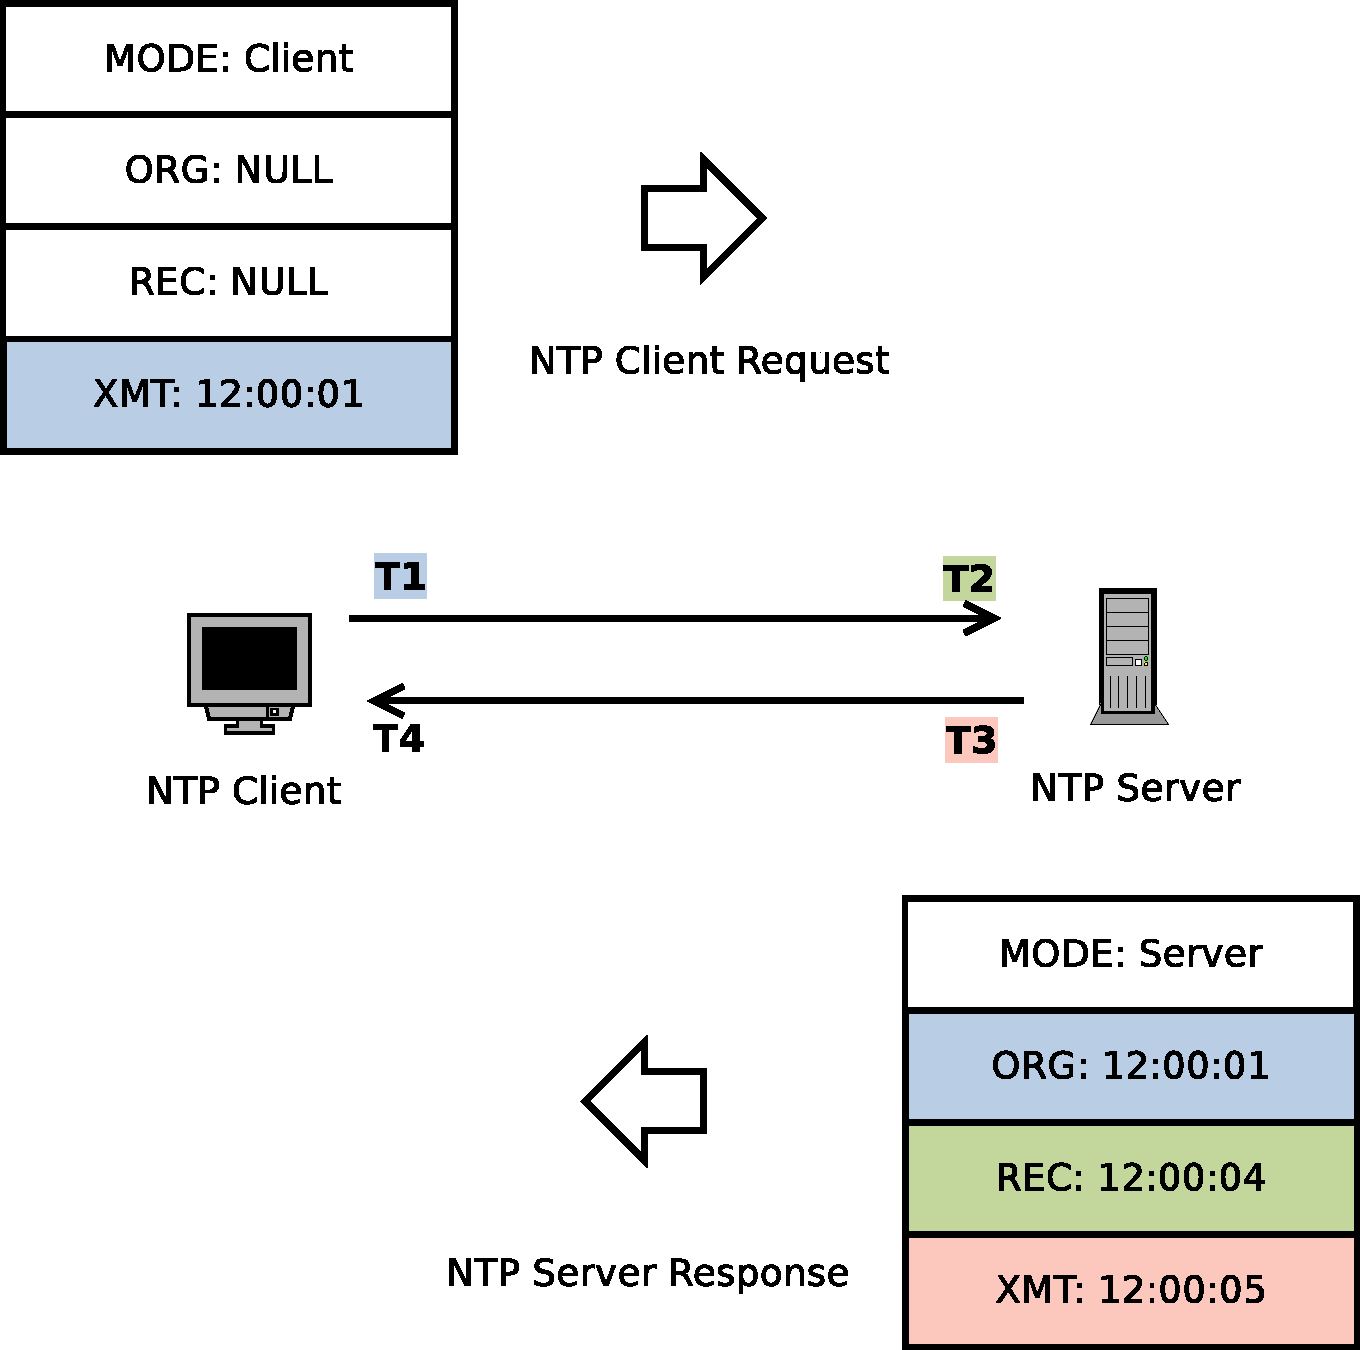
\includegraphics[width=9cm,keepaspectratio]{fig/ntp-client-server.pdf}
	\caption{NTP unicast communication scenario}
	\label{fig:ntp-client-server}
	%\bigskip
\end{figure}
